\begin{frame}
  \frametitle{decision trees}
  
  	{
          \begin{center}
	  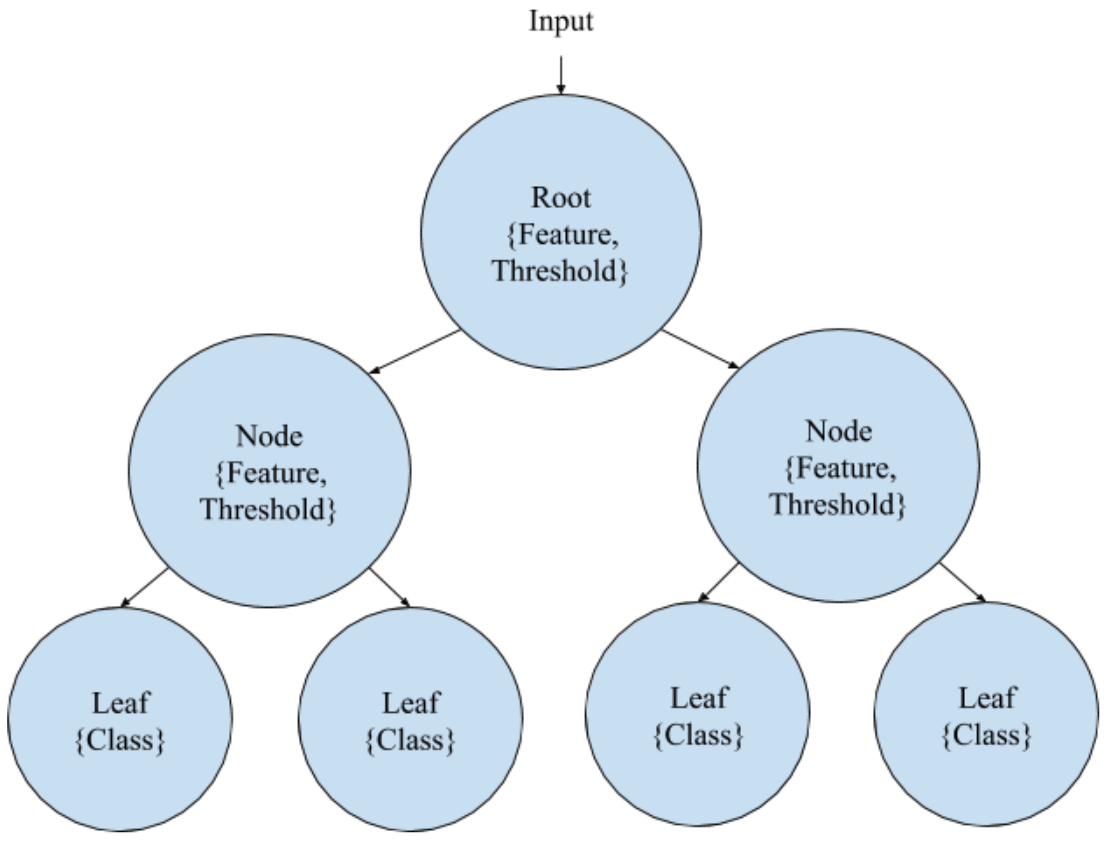
\includegraphics[height=\dimexpr0.8\textheight-0.4in]{decision_tree}
          \end{center}
	}

\end{frame}

\begin{frame}
  \frametitle{training decision trees}
  
  recursive training algorithm:
  %
  \begin{enumerate}
  \item check stopping conditions
    %
    \begin{itemize}
    \item no more features
    \item set is smaller than \code{minLeaf}
    \item all samples in the same class
    \item no feature improves information gain (IG)
    \end{itemize}
  \item iterate over each available feature, perform a line search to approximate the highest IG
  \item recur over the subsets given by splitting at the feature and threshold with the highest IG 
  \end{enumerate}

\begin{equation}
  \mathrm{IG}(X) = \mathrm{H}(X) - \sum_{i=1}^{2} \frac{|S_i|}{|X|} \mathrm{H}(S_i)
\end{equation}

\begin{equation}
  \mathrm{H}(X) = -\sum_{i=1}^n {\mathrm{P}(x_i) \log_2 \mathrm{P}(x_i)}
\end{equation} 
  
\end{frame}